\begin{frame}{Inteligencia Artificial}
%\Huge

		\begin{columns}
		\begin{column}{0.57\textwidth}
		\begin{itemize}
		\item Es un subconjunto de las ciencias de la computación (CC) en donde las máquinas aparentan inteligencia mediante la ejecución de programas. 
		\item Las computadoras intentan resolver tareas que solo son posibles mediante inteligencia humana.
		\item Es una rama muy amplia que cubre muchos aspectos de la vida cotidiana.
		\end{itemize}
		\end{column}
		\begin{column}{0.37\textwidth}  
			\begin{center}
			 %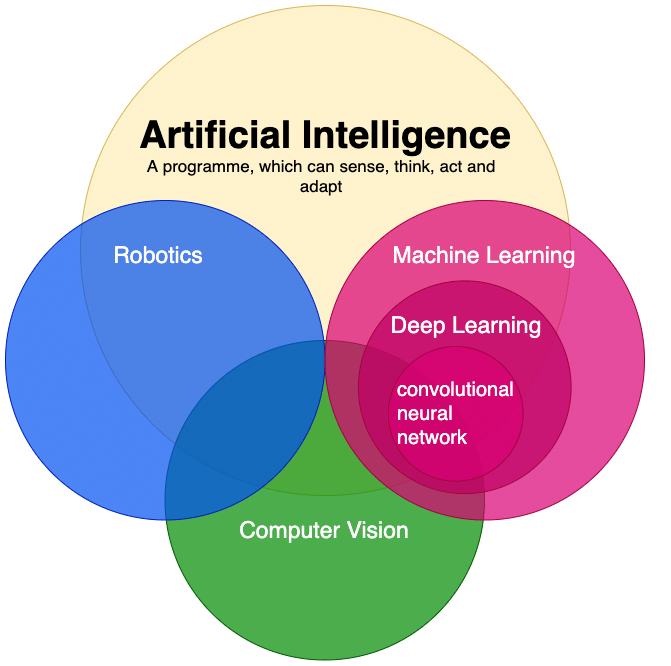
\includegraphics[width=\textwidth]{Figs/Ai1}
\resizebox{\columnwidth}{!}{%
				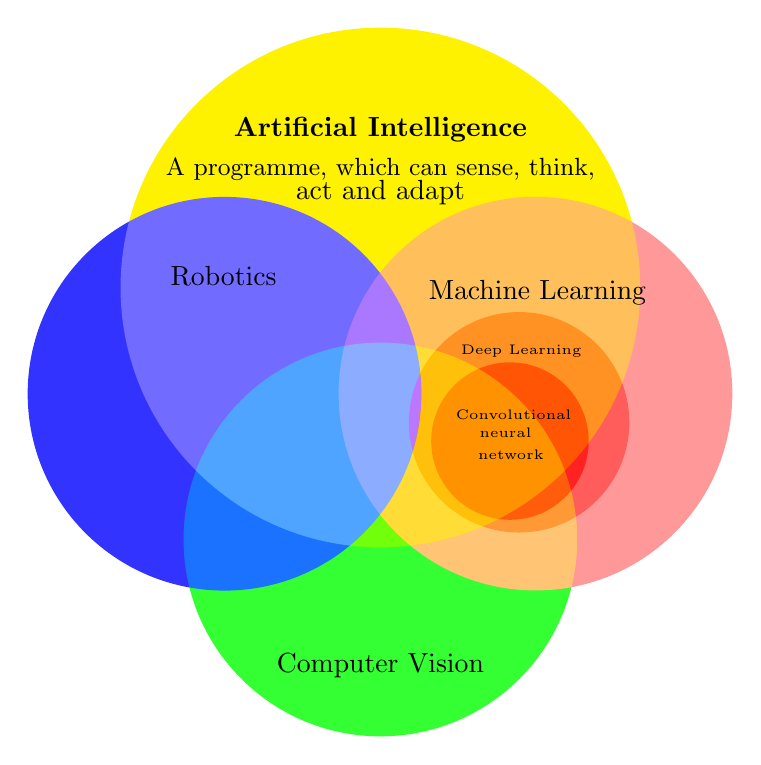
\begin{tikzpicture}
				  \begin{scope}[blend group = soft light]
					\fill[blue!80] (190:2.01) circle (2.5);
					\fill[red!40]  (350:2) circle (2.5);
					\fill[green!80]   ( -90:2.2) circle (2.5);
					\fill[red!100]  (338:1.9) circle (1.4);
					\fill[black!100]  (330:1.9) circle (1);
					\fill[yellow!100]   ( 90:1) circle (3.3);
				   
				   
				  \end{scope}
				  \node at ( 90:3)      {\textbf{Artificial Intelligence}};
				  \node at ( 90:2.5)    {\small A programme, which can sense, think,};
				  \node at ( 90:2.2)    {act and adapt};
				  \node at ( 150:2.3)   {Robotics};
				  \node at ( 385:2.2)   {Machine Learning};
				  \node at ( 366:1.8)   {\tiny Deep Learning};
				  \node at ( 340:1.8)   {\tiny Convolutional};
				  \node at ( 332:1.8)   {\tiny neural};
				  \node at ( 326:2.0)   {\tiny network};
				  \node at ( -90:3.8)   {Computer Vision};
				\end{tikzpicture}
}

			 \end{center}
		\end{column}
	\end{columns}

\end{frame}

